\section{Nuclear Reactors}
\textbf{Light Water Reactor (LWR)} \\
Reactor which uses ordinary water as coolant \\
\textbf{Boiling Water Reactor (BWR)} \\
LWR which allows water to boil in the core. Single loop, steam directly drives generator. Requires powered pumps for circulation and emergency cooling water \\
\textbf{Pressurized Water Reactor (PWR)} \\
LWR where high maintained pressure prevents water boiling. Transfers heat to second water loop which is converted to steam for power \\
\textbf{Canada Deutrium Uranium (CANDU)} \\
$\text{D}_{2}\text{O}$ cooled reactor for better moderation allowing low enriched fuels (nat. uranium). Horizontal fuel bundles, continuous refueling, no outages. \\
\textbf{High Temperature Gas Reactor (HTGR)} \\
High-temperature gas-cooled reactor using pressurized helium. Inherently safe, less fuel \\
\textbf{Liquid Metal Fast Breeder Reactor (LMFBR)} \\
Fast fission, no moderator, typically sodium cooled. Use natural or enriched uranium or plutonium. \\

\subsection{Chain Reactions}
For $\nu$ neutrons released per fission,
\begin{align*}
\eta &= \nu \frac{\sigma_\text{fission}}{\sigma_\text{abs}} \\
\frac{\sigma_\text{fission}}{\sigma_\text{abs}} &= \text{Prob. of Fission per Absorption} \\
\eta > 1 & \quad \text{Chain reaction possible} \\
\eta > 2 & \quad \text{Breeding, creating more fuel, possible}
\end{align*}
Multiplication factor $k$,
\[
k = \frac{\text{\# Neutrons in Generation i}}{\text{\# Neutrons in Generation i+1}}
\]
Can be expressed through the fractional change of neutrons per generation, $\rho$
\[
\rho = (k-1)/k
\]
\begin{align*}
k < 1 & ~~ \rho < 0 & & \enskip \text{Subcritical, reactor shutdown} \\
k = 1 & ~~ \rho = 0 & & \enskip \text{Critical, maintain reactor power} \\
k > 1 & ~~ \rho > 0 & & \enskip \text{Supercritical, reactor startup} 
\end{align*}
With a time $\theta$ between neutron generations, the reactor period $\tau$
\[
\tau = \theta / \ln{k}
\]
Delayed n from fission frag., yield $\beta$, increase $\theta$ \\
Reactor Power increases as
\[
P / P_0 = e^{t \ln{(k)} / \theta}
\]
\begin{align*}
k < 1 + \beta & \qquad \parbox{0.7\linewidth}{Reaction rate controlled by delayed neutrons} \\
k > 1 + \beta & \qquad \parbox{0.7\linewidth}{Prompt super critical, driven by prompt neutrons, uncontrollable}
\end{align*}



\subsection{Six Factor Formula}
\resizebox{\linewidth}{!}{%
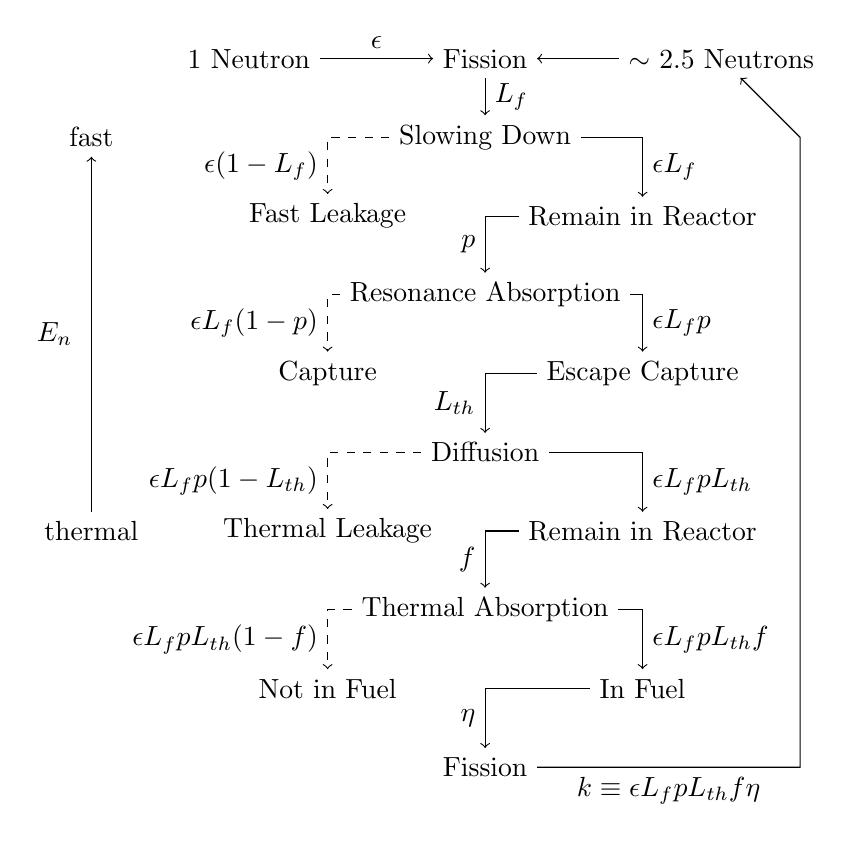
\begin{tikzpicture}
\node (v0) at (-3,0) {1 Neutron};
\node (v1) at (0,0) {Fission};
\draw [->] (v0) edge node[midway, above] {$\epsilon$} (v1);
\node (v3) at (0,-1) {Slowing Down};
\draw [->] (v1) edge node[midway, right] {$L_f$} (v3);
\node (v2) at (-2,-2) {Fast Leakage};
\node (v4) at (2,-2) {Remain in Reactor};
\node (v5) at (0,-3) {Resonance Absorption};
\node (v6) at (-2,-4) {Capture};
\node (v7) at (2,-4) {Escape Capture};
\node (v8) at (0,-5) {Diffusion};
\node (v9) at (-2,-6) {Thermal Leakage};
\node (v10) at (2,-6) {Remain in Reactor};
\node (v11) at (0,-7) {Thermal Absorption};
\node (v12) at (-2,-8) {Not in Fuel};
\node (v13) at (2,-8) {In Fuel};
\node (v14) at (0,-9) {Fission};
\node (v15) at (3,0) {$\sim$ 2.5 Neutrons};
\node (v16) at (-5, -6) {thermal};
\node (v17) at (-5, -1) {fast};
\draw [->, dashed] (v3) -- (-2,-1) -- node[midway, left] {$\epsilon (1-L_f)$} (v2);
\draw [->] (v3) -- (2,-1) -- node[midway, right] {$\epsilon L_f$} (v4);
\draw [->] (v4) -- (0,-2) -- node[midway, left] {$p$} (v5);
\draw [->, dashed] (v5) -- (-2,-3) -- node[midway, left] {$\epsilon L_f (1-p)$} (v6);
\draw [->] (v5) -- (2,-3) -- node[midway, right] {$\epsilon L_f p$} (v7);
\draw [->] (v7) -- (0,-4) -- node[midway, left] {$L_{th}$} (v8);
\draw [->, dashed] (v8) -- (-2,-5) -- node[midway, left] {$\epsilon L_f p (1-L_{th})$} (v9);
\draw [->] (v8) -- (2,-5) -- node[midway, right] {$\epsilon L_f p L_{th}$} (v10);
\draw [->] (v10) -- (0,-6) -- node[midway, left] {$f$} (v11);
\draw [->, dashed] (v11) -- (-2,-7) -- node[midway, left] {$\epsilon L_f p L_{th} (1-f)$} (v12);
\draw [->] (v11) -- (2,-7) -- node[midway, right] {$\epsilon L_f p L_{th} f$} (v13);
\draw [->] (v13) -- (0,-8) -- node[midway, left] {$\eta$} (v14);
\draw [->] (v15) -- (v1);
\draw [->] (v14) -- node[midway, below] {$k \equiv \epsilon L_f p L_{th} f \eta$} (4,-9) -- (4,-1) -- (v15);
\draw [->] (v16) -- (v17) node[midway, left] {$E_n~$};
\end{tikzpicture}
}
\[
k \equiv \epsilon ~ p ~ f ~ \eta ~ L_f ~ L_t
\]
\begin{align*}
\epsilon & \quad \text{fast fission factor} \\
p & \quad \text{resonance escape prob} \\
f & \quad \text{thermal utilization factor} \\
\eta & \quad \text{\# neutrons per abs. in fuel} \\
L_f & \quad \text{fast non-leak prob} \\
L_t & \quad \text{thermal non-leak prob}
\end{align*}
\[
f = \frac{\Sigma_a^\text{fuel}}{\Sigma_a^\text{all mat}} \quad \eta = \frac{\nu \sigma_\text{fiss}^\text{fuel}}{\sigma_\text{abs}^\text{fuel}}
\]

For infinite reactor with no leakage
\[
k_\infty = \epsilon ~ p ~ f ~ \eta
\]

\subsection{Reactor Kinetics}
\[
k = \frac{P(T)}{L(T)} = \frac{\text{Neutron Production Rate}}{\text{Neutron Loss Rate}}
\]
Neutron lifetime $l$ ($\theta$) and reactor period $T$ ($\tau$)
\[
l = \frac{N(T)}{L(T)} \qquad T = \frac{l}{k-1}
\]
\[
N(T) = N_0 e^{t/T}
\]

\subsection{Neutron Diffusion}
\begin{gather*}
-D \nabla^2 \Phi(\vec{r}) + \Sigma_R \Phi(\vec{r}) = S(\Phi(\vec{r})) \\
S(\Phi(\vec{r})) = \nu \Sigma_f \Phi(\vec{r}) \\
D = 1 / 3 ~ \Sigma_{tr} \\
\Sigma_{tr} = \Sigma_T - \mu_0 \Sigma_s \\
L = \sqrt{D / \Sigma_a}
k = \frac{B_m^2}{B_g^2}
\end{gather*}